% !TeX root = ..//diffgeo_main.tex

Unser nächster Schritt ist es nun die Parallelverschiebung zu definieren.
Auf dem Weg dorthin ist unser erstes Ziel zunächst die kovariante Ableitung von Schnitten längs einer Abbildung zu definieren.
\begin{enumerate}
\item Zu Schnitten längs einer Abbildung:
\begin{align}
\label{diag:schnittf}
\begin{xy}
  \xymatrix@=0.2\linewidth{
          &   E \ar[d]_{\pi} \\
      \mfka \ar[ur]^{s^\text{{\begin{tiny}$\mfka$\end{tiny}}}}  \ar[r]_f  &   \mfk
  }
\end{xy}
\end{align}
Eine Abbildung $s^\text{{\begin{tiny}$\mfka$\end{tiny}}} : \mfka \to E$ heißt Schnitt längs $f: \mfka \to \mfk$ falls:
\begin{enumerate}
  \item[i)]  $s^\text{{\begin{tiny}$\mfka$\end{tiny}}}$ ist glatt
  \item[ii)]  Das Diagramm \ref{diag:schnittf} kommutiert: $f = \pi \circ s^\text{{\begin{tiny}$\mfka$\end{tiny}}}$
\end{enumerate}
Notation: $\Gamma_f (E)$\\
\textbf{Wichtiger Spezialfall}: $\mfka = I$, das heißt $f$ ist eine Kurve falls $E = T\mfk$
\begin{figure}[H]
\centering
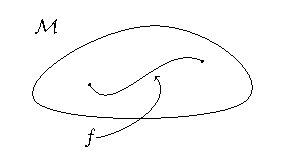
\includegraphics[width=0.4\linewidth]{figures/tikz/curve_on_manifold.pdf}
\label{img:curve_on_manifold}
\caption{Kurve $f$ auf einer Mannigfaltigkeit}
\end{figure} 
Hier sieht das Diagramm dann wie folgt aus:
\begin{align}
\begin{xy}
  \xymatrix@=0.2\linewidth{
          &   T\mfk \ar[d]_{\pi} \\
      I \ar[ur]^{s^I} \ar[r]_f  &   \mfk
  }
\end{xy}
\end{align}
\item Wollen $\covd: \mathfrak{X}(\mfka) \times \Gamma_f (E) \to \Gamma_f (E)$.
\end{enumerate}

\begin{defs}[Kovariante Ableitung längs eines Schnittes]
Sei $\phi = (s_1, \dots, s_k)$ ein lokaler Rahmen von $E$ über $U$ und $s \in \Gamma_f (U)$. 
Dann ist:
\begin{align}
s = \sum^{k}_{i=1} \sigma_i s_i \circ f
\end{align}
Wir definieren die kovariante Ableitung längs $f$ als:
\begin{align}
\covd^{f}_X s &= \sum^k_{j=1} \left( X(\sigma_j) + \sum^k_{i=1} \omega_{ij}(f_\ast X)\sigma_i \right) s_j \circ f\\
&= X(\sigma) + (f^\ast \omega)(X) \sigma
\end{align}
Die Wohldefinertheit soll als Übung gezeigt werden.
\end{defs}
\begin{satz}
Die kovariante Ableitung längs $f$
\begin{align*}
\covd^f: \mathfrak{X}(\mfka) \times \Gamma_f (E) \to \Gamma_f (E),
\end{align*}
ist tensoriell im ersten Argument und derivativ im zweiten Argument.
\end{satz}
Wenn wir die Schnitte $\Gamma_f (E)$ mit $\Gamma(f^\ast E)$ identifizieren, dann erhalten wir den zurückgezogenen Zusammenhang
\begin{align}
f^\ast \covd : \mathfrak{X}(\mfka) \times\Gamma(f^\ast E) \to \Gamma(f^\ast E).
\end{align}
\begin{satz}
Sei $s^\text{{\begin{tiny}$\mfk$\end{tiny}}} \in \Gamma(E)$, $q \in \mfka$ und $v\in T_q \mfka$.
Dann gilt:
\begin{align}
\covd^f_v (s^\text{{\begin{tiny}$\mfk$\end{tiny}}} \circ f) = \covd_{f^\ast v} s^\text{{\begin{tiny}$\mfk$\end{tiny}}}
\end{align}
Die wichtigste Situation ist hierbei der Fall der Kurven also mit $\mfka = I$ und $E = T\mfk$.
Hier gilt nämlich
\begin{align}
\covd_t s := \covd^c_{\pdv{t}} s.
\end{align}
\end{satz}
\begin{bem}
Sei $c$ so gewählt, dass $\dot{c}(t) = 0$, das heißt $c(t)=p$.\\
\textbf{Achtung:} $\covd_t s$ kann ungleich Null sein, selbst wenn $\dot{c}(t) = 0$.\\
Zum Beispiel: $c(t)=p$ und $s \in \Gamma_c (E)$, dann muss $s(t) \in E_p$ nicht konstant sein.
%Dann ist $\covd_t s = \pdv{t} s $ Ableitung um $s(1)$ als Abbildung in $E_p \cong \R^k$.
\end{bem}
Als nächstes wollen wir nun die kovariante Ableitung längs von Kurven verwenden, um die Parallelverschiebung zu definieren.
\begin{defs}[Parallelität]
Sei $c: I \to \mfk$ eine glatte Kurve und $(E, \pi, \mfk)$ ein Vektorbündel.
Ein Schnitt $s^I \in \Gamma_c (E)$ heißt parallel längs $c$, falls 
\begin{align}
\covd^c_t s = 0.
\end{align}
\end{defs}
\begin{bem}
Wenn $s_1$ und $s_2$ parallel sind, so ist auch $\alpha s_1 + \beta s_1$ ($\forall \alpha, \beta \in \R$) parallel.
\end{bem}
In einem lokalen Rahmen bedeutet $\covd^c_t s = 0$:
\begin{align}
\dot{\sigma} + \omega(\dot{c}) \sigma = 0.
\end{align}
Dies ist eine gewöhnliche Differentialgleichung erster Ordnung.
\begin{lem}
Sei $t_0 \in I$ und $X \in E_{c(t_0)}$ dann existiert genau ein paralleler Schnitt $s$ längs $c$ mit $s(t_0) = x$.
\end{lem}
Sei $c$ eine glatte Kurve mit $c(t_0) = p$ und $c(t_1)=q$ ($t_0, t_1 \in I$).
Setze $P_c(x) = s(t_1)$ wobei $s$ der eindeutig bestimmte parallele Schnitt längs $c$ mit $s(t_0) = x$ ist.
\begin{defs}[Parallelverschiebung]
$P_c : E_p \to E_q$ heißt Parallelverschiebung längs $c$.
\begin{figure}[H]
\centering
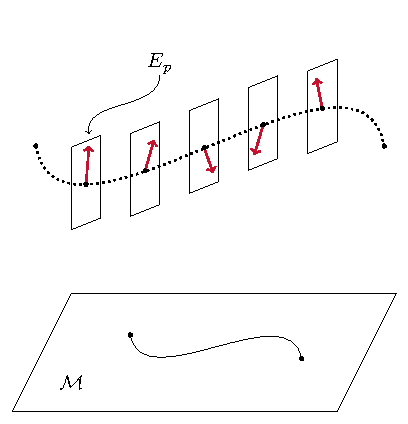
\includegraphics[width=0.7\linewidth]{figures/tikz/parallel_shift_dgl.pdf}
\label{img:parallel_shift:dgl}
\caption{Parallelverschiebung}
\end{figure} 
\end{defs}
\begin{lem}
\label{lem:BasisVB}
Sei $t_0 \in I$ und seien $s_1, \dots, s_k$ parallele Schnitte längs $c$.
Falls $(s^I_1 (t_0), \dots, s^I_k (t_0))$ eine Basis von $E_{c(t_0)}$ ist, so ist $(s^I_1 (t), \dots, s^I_k (t))$ eine Basis von $E_{c(t)}$ für alle $t \in I$.
\end{lem}
\begin{bew}[Lemma \ref{lem:BasisVB}]
\begin{align*}
s^I_i (t) = P_c s^I_i (t_0)
\end{align*}
Da $P$ invertierbar ist folgt die Aussage.% , dass $s(^I_1 (t), \dots, s^I_k (t))$
\end{bew}
\begin{defs}[Paralleler Rahmen]
Ein $k$-Tupel von Schnitten $\phi = (s_1, \dots, s_k)$ längs $c$ heißt Rahmen von $E$ längs $c$, falls $(s_1(t), \dots s_k(t))$ eine Basis von $E_{c(t)}$ für alle $t \in I$ ist.
$\phi = (s_1, \dots, s_k)$ heißt paralleler Rahmen, falls alle $s_i$ parallel sind.
\end{defs}
\textit{Warum sind parallele Rahmen für uns interessant?}\\
Wir betrachten den parallelen Rahmen $\phi = (s_1, \dots, s_k)$ und sei $s \in \Gamma_c (E)$.
Das heißt 
\begin{align*}
s= \sum^{k}_{i=1} \sigma_i s_i.
\end{align*}
Damit erhalten wir für die kovariante Ableitung:
\begin{align}
\covd_t s &= \sum^{k}_{i=1} \covd_t (\sigma_i s_i)\\
&= \sum^{k}_{i=1} (\partial_t \sigma_i) s_i. 
\end{align}
Bezüglich des parallelen Rahmens ist die kovariante Ableitung also gerade die Standardableitung.
\begin{bem}
Parallelverschiebung kann man allgemein längs Stückweiser glatter Kurven $c$ defineren.
\end{bem}


